\documentclass[]{article}
\usepackage{lmodern}
\usepackage{amssymb,amsmath}
\usepackage{ifxetex,ifluatex}
\usepackage{fixltx2e} % provides \textsubscript
\ifnum 0\ifxetex 1\fi\ifluatex 1\fi=0 % if pdftex
  \usepackage[T1]{fontenc}
  \usepackage[utf8]{inputenc}
\else % if luatex or xelatex
  \ifxetex
    \usepackage{mathspec}
  \else
    \usepackage{fontspec}
  \fi
  \defaultfontfeatures{Ligatures=TeX,Scale=MatchLowercase}
\fi
% use upquote if available, for straight quotes in verbatim environments
\IfFileExists{upquote.sty}{\usepackage{upquote}}{}
% use microtype if available
\IfFileExists{microtype.sty}{%
\usepackage{microtype}
\UseMicrotypeSet[protrusion]{basicmath} % disable protrusion for tt fonts
}{}
\usepackage[margin=1in]{geometry}
\usepackage{hyperref}
\hypersetup{unicode=true,
            pdftitle={Angewandte Forschungsmethodik I: Strukturgleichungsmodellierung I (SS 18)},
            pdfauthor={Übungsblatt 3: Fabio Votta, 2891518},
            pdfborder={0 0 0},
            breaklinks=true}
\urlstyle{same}  % don't use monospace font for urls
\usepackage{color}
\usepackage{fancyvrb}
\newcommand{\VerbBar}{|}
\newcommand{\VERB}{\Verb[commandchars=\\\{\}]}
\DefineVerbatimEnvironment{Highlighting}{Verbatim}{commandchars=\\\{\}}
% Add ',fontsize=\small' for more characters per line
\usepackage{framed}
\definecolor{shadecolor}{RGB}{248,248,248}
\newenvironment{Shaded}{\begin{snugshade}}{\end{snugshade}}
\newcommand{\KeywordTok}[1]{\textcolor[rgb]{0.13,0.29,0.53}{\textbf{#1}}}
\newcommand{\DataTypeTok}[1]{\textcolor[rgb]{0.13,0.29,0.53}{#1}}
\newcommand{\DecValTok}[1]{\textcolor[rgb]{0.00,0.00,0.81}{#1}}
\newcommand{\BaseNTok}[1]{\textcolor[rgb]{0.00,0.00,0.81}{#1}}
\newcommand{\FloatTok}[1]{\textcolor[rgb]{0.00,0.00,0.81}{#1}}
\newcommand{\ConstantTok}[1]{\textcolor[rgb]{0.00,0.00,0.00}{#1}}
\newcommand{\CharTok}[1]{\textcolor[rgb]{0.31,0.60,0.02}{#1}}
\newcommand{\SpecialCharTok}[1]{\textcolor[rgb]{0.00,0.00,0.00}{#1}}
\newcommand{\StringTok}[1]{\textcolor[rgb]{0.31,0.60,0.02}{#1}}
\newcommand{\VerbatimStringTok}[1]{\textcolor[rgb]{0.31,0.60,0.02}{#1}}
\newcommand{\SpecialStringTok}[1]{\textcolor[rgb]{0.31,0.60,0.02}{#1}}
\newcommand{\ImportTok}[1]{#1}
\newcommand{\CommentTok}[1]{\textcolor[rgb]{0.56,0.35,0.01}{\textit{#1}}}
\newcommand{\DocumentationTok}[1]{\textcolor[rgb]{0.56,0.35,0.01}{\textbf{\textit{#1}}}}
\newcommand{\AnnotationTok}[1]{\textcolor[rgb]{0.56,0.35,0.01}{\textbf{\textit{#1}}}}
\newcommand{\CommentVarTok}[1]{\textcolor[rgb]{0.56,0.35,0.01}{\textbf{\textit{#1}}}}
\newcommand{\OtherTok}[1]{\textcolor[rgb]{0.56,0.35,0.01}{#1}}
\newcommand{\FunctionTok}[1]{\textcolor[rgb]{0.00,0.00,0.00}{#1}}
\newcommand{\VariableTok}[1]{\textcolor[rgb]{0.00,0.00,0.00}{#1}}
\newcommand{\ControlFlowTok}[1]{\textcolor[rgb]{0.13,0.29,0.53}{\textbf{#1}}}
\newcommand{\OperatorTok}[1]{\textcolor[rgb]{0.81,0.36,0.00}{\textbf{#1}}}
\newcommand{\BuiltInTok}[1]{#1}
\newcommand{\ExtensionTok}[1]{#1}
\newcommand{\PreprocessorTok}[1]{\textcolor[rgb]{0.56,0.35,0.01}{\textit{#1}}}
\newcommand{\AttributeTok}[1]{\textcolor[rgb]{0.77,0.63,0.00}{#1}}
\newcommand{\RegionMarkerTok}[1]{#1}
\newcommand{\InformationTok}[1]{\textcolor[rgb]{0.56,0.35,0.01}{\textbf{\textit{#1}}}}
\newcommand{\WarningTok}[1]{\textcolor[rgb]{0.56,0.35,0.01}{\textbf{\textit{#1}}}}
\newcommand{\AlertTok}[1]{\textcolor[rgb]{0.94,0.16,0.16}{#1}}
\newcommand{\ErrorTok}[1]{\textcolor[rgb]{0.64,0.00,0.00}{\textbf{#1}}}
\newcommand{\NormalTok}[1]{#1}
\usepackage{graphicx,grffile}
\makeatletter
\def\maxwidth{\ifdim\Gin@nat@width>\linewidth\linewidth\else\Gin@nat@width\fi}
\def\maxheight{\ifdim\Gin@nat@height>\textheight\textheight\else\Gin@nat@height\fi}
\makeatother
% Scale images if necessary, so that they will not overflow the page
% margins by default, and it is still possible to overwrite the defaults
% using explicit options in \includegraphics[width, height, ...]{}
\setkeys{Gin}{width=\maxwidth,height=\maxheight,keepaspectratio}
\IfFileExists{parskip.sty}{%
\usepackage{parskip}
}{% else
\setlength{\parindent}{0pt}
\setlength{\parskip}{6pt plus 2pt minus 1pt}
}
\setlength{\emergencystretch}{3em}  % prevent overfull lines
\providecommand{\tightlist}{%
  \setlength{\itemsep}{0pt}\setlength{\parskip}{0pt}}
\setcounter{secnumdepth}{0}
% Redefines (sub)paragraphs to behave more like sections
\ifx\paragraph\undefined\else
\let\oldparagraph\paragraph
\renewcommand{\paragraph}[1]{\oldparagraph{#1}\mbox{}}
\fi
\ifx\subparagraph\undefined\else
\let\oldsubparagraph\subparagraph
\renewcommand{\subparagraph}[1]{\oldsubparagraph{#1}\mbox{}}
\fi

%%% Use protect on footnotes to avoid problems with footnotes in titles
\let\rmarkdownfootnote\footnote%
\def\footnote{\protect\rmarkdownfootnote}

%%% Change title format to be more compact
\usepackage{titling}

% Create subtitle command for use in maketitle
\newcommand{\subtitle}[1]{
  \posttitle{
    \begin{center}\large#1\end{center}
    }
}

\setlength{\droptitle}{-2em}
  \title{Angewandte Forschungsmethodik I: Strukturgleichungsmodellierung I (SS
18)}
  \pretitle{\vspace{\droptitle}\centering\huge}
  \posttitle{\par}
  \author{Übungsblatt 3: Fabio Votta, 2891518}
  \preauthor{\centering\large\emph}
  \postauthor{\par}
  \predate{\centering\large\emph}
  \postdate{\par}
  \date{07/05/2018}

\usepackage{pdflscape}
\usepackage{booktabs}

\begin{document}
\maketitle

\section{Recoding}\label{recoding}

\begin{Shaded}
\begin{Highlighting}[]
\NormalTok{allbus }\OperatorTok\StringTok{ }
\StringTok{  }\KeywordTok{select}\NormalTok{(}\OperatorTok{-}\NormalTok{mn11}\OperatorTok{:-}\NormalTok{mn21) }\OperatorTok\StringTok{ }\CommentTok{#select(mm05) %>% table()}
\StringTok{  }\KeywordTok{mutate}\NormalTok{(}\DataTypeTok{mm02 =} \DecValTok{8} \OperatorTok{-}\StringTok{ }\NormalTok{mm02) }\OperatorTok\StringTok{ }
\StringTok{  }\KeywordTok{mutate}\NormalTok{(}\DataTypeTok{mm05 =} \DecValTok{8} \OperatorTok{-}\StringTok{ }\NormalTok{mm05) }\OperatorTok\StringTok{ }
\StringTok{  }\KeywordTok{select}\NormalTok{(mm01}\OperatorTok{:}\NormalTok{mm06, Alter, Bildung, Geschlecht)}
\end{Highlighting}
\end{Shaded}

\section{Imputation}\label{imputation}

\begin{Shaded}
\begin{Highlighting}[]
\NormalTok{mice_allbus <-}\StringTok{ }\KeywordTok{mice}\NormalTok{(allbus, }\DataTypeTok{method =} \StringTok{"norm.nob"}\NormalTok{, }\DataTypeTok{m =} \DecValTok{1}\NormalTok{)}

\NormalTok{imp_allbus <-}\StringTok{ }\KeywordTok{complete}\NormalTok{(mice_allbus)}

\KeywordTok{names}\NormalTok{(imp_allbus) <-}\StringTok{ }\KeywordTok{paste0}\NormalTok{(}\KeywordTok{names}\NormalTok{(imp_allbus), }\StringTok{"_imp"}\NormalTok{)}
\end{Highlighting}
\end{Shaded}

\section{Merging}\label{merging}

\begin{Shaded}
\begin{Highlighting}[]
\NormalTok{combined_allbus <-}\StringTok{ }\NormalTok{allbus }\OperatorTok\StringTok{ }
\StringTok{  }\KeywordTok{cbind}\NormalTok{(imp_allbus) }
  
\NormalTok{combined_allbus }\OperatorTok\StringTok{ }
\StringTok{  }\NormalTok{sjmisc}\OperatorTok{::}\KeywordTok{descr}\NormalTok{() }\OperatorTok\StringTok{ }
\StringTok{  }\KeywordTok{as.data.frame}\NormalTok{() }\OperatorTok\StringTok{ }
\StringTok{  }\KeywordTok{select}\NormalTok{(}\OperatorTok{-}\NormalTok{type, }\OperatorTok{-}\NormalTok{label, }\OperatorTok{-}\NormalTok{se}\OperatorTok{:-}\NormalTok{trimmed) }\OperatorTok\StringTok{ }
\StringTok{  }\KeywordTok{arrange}\NormalTok{(variable) }\OperatorTok\StringTok{ }
\StringTok{  }\NormalTok{knitr}\OperatorTok{::}\KeywordTok{kable}\NormalTok{()}
\end{Highlighting}
\end{Shaded}

\section{Correlation Matrices}\label{correlation-matrices}

\begin{Shaded}
\begin{Highlighting}[]
\NormalTok{ggheatmap <-}\StringTok{ }\ControlFlowTok{function}\NormalTok{(.data) \{}
  
 \KeywordTok{library}\NormalTok{(reshape2)}
 
\NormalTok{ cormat <-}\StringTok{ }\KeywordTok{round}\NormalTok{(}\KeywordTok{cor}\NormalTok{(.data, }\DataTypeTok{use =} \StringTok{"pairwise.complete.obs"}\NormalTok{),}\DecValTok{3}\NormalTok{)}
 
 \CommentTok{# Get upper triangle of the correlation matrix}
\NormalTok{ get_upper_tri <-}\StringTok{ }\ControlFlowTok{function}\NormalTok{(cormat)\{}
\NormalTok{     cormat[}\KeywordTok{lower.tri}\NormalTok{(cormat)] <-}\StringTok{ }\OtherTok{NA}
     \KeywordTok{return}\NormalTok{(cormat)}
\NormalTok{   \}}
 
\NormalTok{ reorder_cormat <-}\StringTok{ }\ControlFlowTok{function}\NormalTok{(cormat)\{}
 \CommentTok{# Use correlation between variables as distance}
\NormalTok{ dd <-}\StringTok{ }\KeywordTok{as.dist}\NormalTok{((}\DecValTok{1}\OperatorTok{-}\NormalTok{cormat)}\OperatorTok{/}\DecValTok{2}\NormalTok{)}
\NormalTok{ hc <-}\StringTok{ }\KeywordTok{hclust}\NormalTok{(dd)}
\NormalTok{ cormat <-}\StringTok{ }\NormalTok{cormat[hc}\OperatorTok{$}\NormalTok{order, hc}\OperatorTok{$}\NormalTok{order]}
\NormalTok{ \}}
 
 \CommentTok{# Reorder the correlation matrix}
 \CommentTok{#cormat <- reorder_cormat(cormat)}
\NormalTok{ upper_tri <-}\StringTok{ }\KeywordTok{get_upper_tri}\NormalTok{(cormat)}
 \CommentTok{# Melt the correlation matrix}
\NormalTok{ melted_cormat <-}\StringTok{ }\KeywordTok{melt}\NormalTok{(upper_tri, }\DataTypeTok{na.rm =} \OtherTok{TRUE}\NormalTok{) }\OperatorTok\StringTok{ }
\StringTok{   }\KeywordTok{mutate}\NormalTok{(}\DataTypeTok{value =} \KeywordTok{sprintf}\NormalTok{(}\StringTok{'%.2f'}\NormalTok{, value, }\DecValTok{2}\NormalTok{)) }\OperatorTok\StringTok{ }
\StringTok{   }\KeywordTok{mutate}\NormalTok{(}\DataTypeTok{value =} \KeywordTok{as.numeric}\NormalTok{(value))}
 \CommentTok{# Create a ggheatmap}
 \KeywordTok{ggplot}\NormalTok{(melted_cormat, }\KeywordTok{aes}\NormalTok{(Var2, Var1, }\DataTypeTok{fill =}\NormalTok{ value)) }\OperatorTok{+}
\StringTok{  }\KeywordTok{geom_tile}\NormalTok{(}\DataTypeTok{color =} \StringTok{"white"}\NormalTok{)}\OperatorTok{+}
\StringTok{  }\KeywordTok{scale_fill_gradient2}\NormalTok{(}\DataTypeTok{low =} \StringTok{"blue"}\NormalTok{, }\DataTypeTok{high =} \StringTok{"red"}\NormalTok{, }\DataTypeTok{mid =} \StringTok{"white"}\NormalTok{, }
    \DataTypeTok{midpoint =} \DecValTok{0}\NormalTok{, }\DataTypeTok{limit =} \KeywordTok{c}\NormalTok{(}\OperatorTok{-}\DecValTok{1}\NormalTok{,}\DecValTok{1}\NormalTok{), }\DataTypeTok{space =} \StringTok{"Lab"}\NormalTok{, }
     \DataTypeTok{name=}\StringTok{"Pearson Correlation}\CharTok{\textbackslash{}n}\StringTok{"}\NormalTok{) }\OperatorTok{+}
\StringTok{  }\NormalTok{ggthemes}\OperatorTok{::}\KeywordTok{theme_hc}\NormalTok{()}\OperatorTok{+}\StringTok{ }\CommentTok{# minimal theme}
\StringTok{  }\KeywordTok{theme}\NormalTok{(}\DataTypeTok{axis.text.x =} \KeywordTok{element_text}\NormalTok{(}\DataTypeTok{angle =} \DecValTok{45}\NormalTok{, }\DataTypeTok{vjust =} \DecValTok{1}\NormalTok{, }
     \DataTypeTok{size =} \DecValTok{12}\NormalTok{, }\DataTypeTok{hjust =} \DecValTok{1}\NormalTok{))}\OperatorTok{+}
\StringTok{ }\CommentTok{# coord_fixed()  + }
\StringTok{ }\KeywordTok{geom_text}\NormalTok{(}\KeywordTok{aes}\NormalTok{(Var2, Var1, }\DataTypeTok{label =}\NormalTok{ value), }\DataTypeTok{color =} \StringTok{"black"}\NormalTok{, }\DataTypeTok{size =} \DecValTok{4}\NormalTok{) }\OperatorTok{+}
\StringTok{ }\KeywordTok{theme}\NormalTok{(}
   \DataTypeTok{axis.title.x =} \KeywordTok{element_blank}\NormalTok{(),}
   \DataTypeTok{axis.title.y =} \KeywordTok{element_blank}\NormalTok{(),}
   \DataTypeTok{panel.grid.major =} \KeywordTok{element_blank}\NormalTok{(),}
   \DataTypeTok{panel.border =} \KeywordTok{element_blank}\NormalTok{(),}
   \DataTypeTok{panel.background =} \KeywordTok{element_blank}\NormalTok{(),}
   \DataTypeTok{axis.ticks =} \KeywordTok{element_blank}\NormalTok{(),}
   \DataTypeTok{legend.justification =} \KeywordTok{c}\NormalTok{(}\DecValTok{1}\NormalTok{, }\DecValTok{0}\NormalTok{),}
   \DataTypeTok{legend.position =} \KeywordTok{c}\NormalTok{(}\FloatTok{0.7}\NormalTok{, }\FloatTok{0.8}\NormalTok{),}
   \DataTypeTok{legend.title =} \KeywordTok{element_text}\NormalTok{(}\DataTypeTok{size =} \DecValTok{20}\NormalTok{),}
   \DataTypeTok{axis.ticks.length =} \KeywordTok{unit}\NormalTok{(}\DecValTok{2}\NormalTok{, }\StringTok{"cm"}\NormalTok{),}
   \DataTypeTok{legend.direction =} \StringTok{"horizontal"}\NormalTok{)}\OperatorTok{+}
\StringTok{   }\KeywordTok{guides}\NormalTok{(}\DataTypeTok{fill =} \KeywordTok{guide_colorbar}\NormalTok{(}\DataTypeTok{barwidth =} \DecValTok{30}\NormalTok{, }\DataTypeTok{barheight =} \FloatTok{1.5}\NormalTok{,}
                 \DataTypeTok{title.position =} \StringTok{"top"}\NormalTok{, }\DataTypeTok{title.hjust =} \FloatTok{0.5}\NormalTok{))}
\NormalTok{\}}

\KeywordTok{ggheatmap}\NormalTok{(combined_allbus)}
\end{Highlighting}
\end{Shaded}

\begin{center}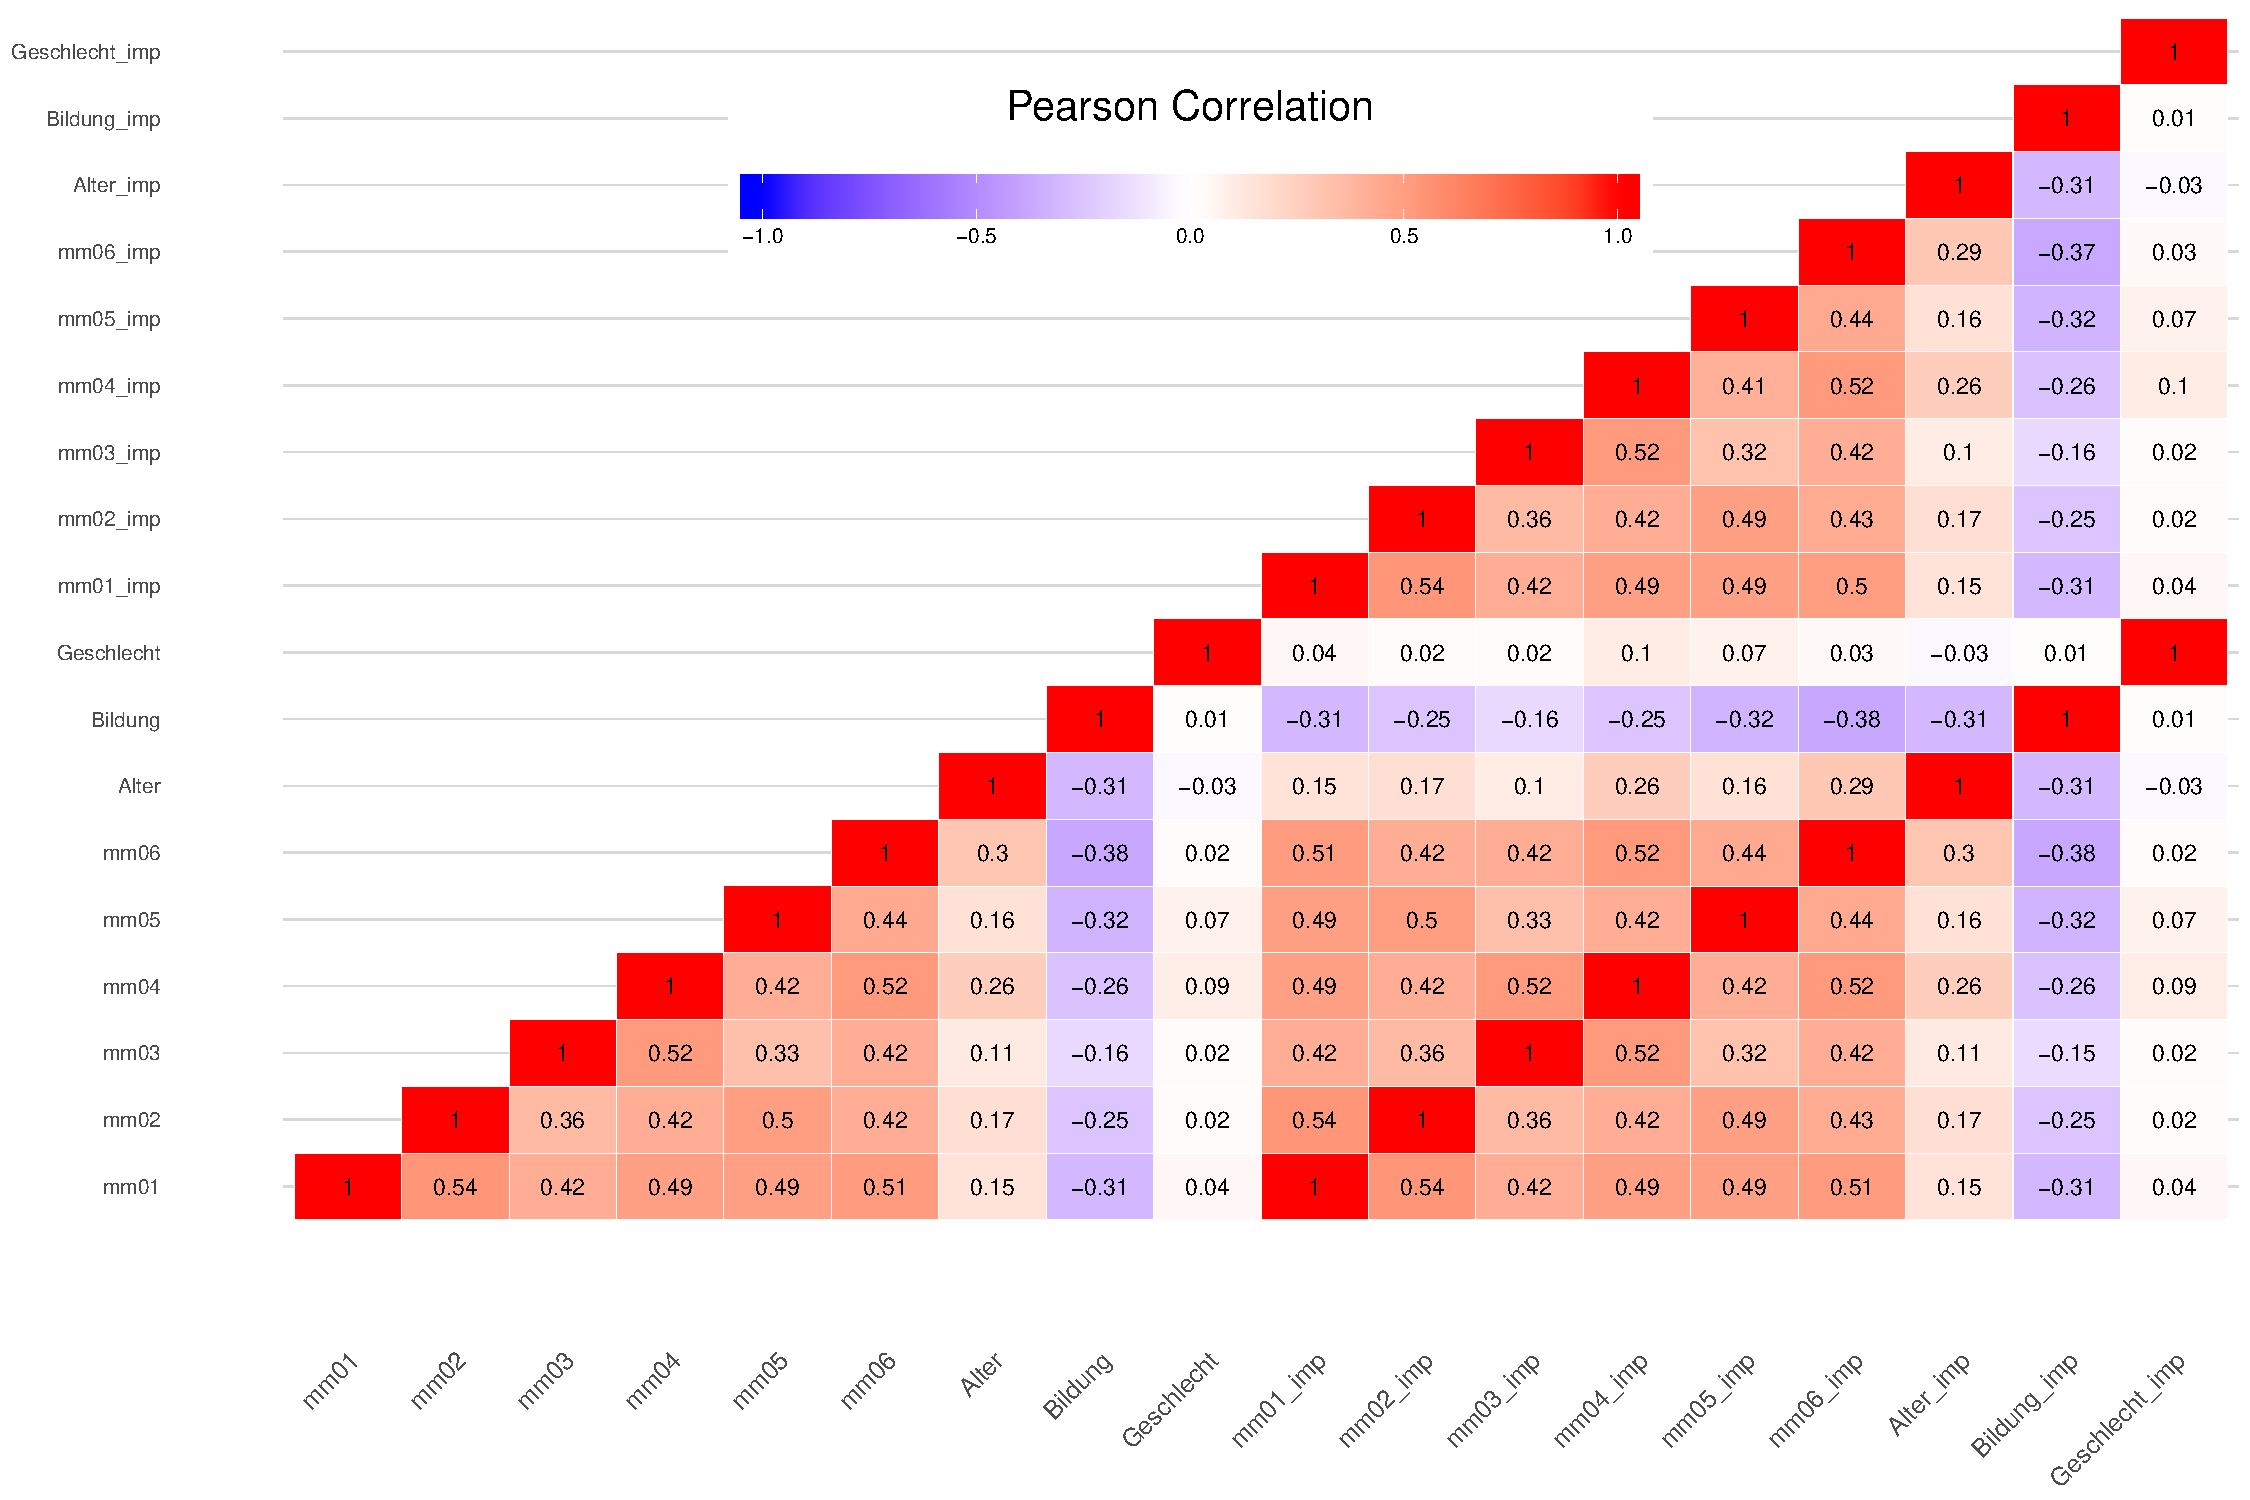
\includegraphics{ua3_files/figure-latex/unnamed-chunk-3-1} \end{center}


\end{document}
